\pagebreak
\section{Approach}

\picHereWidth{grasp_pipeline}{Pipeline for object grasping.}{fig:grasp_pipeline}{\textwidth}

Figure \ref{fig:grasp_pipeline} illustrates the main components of the object grasping pipeline implemented on the HSR.
This section will detail the implementation of each component.

\subsection{Object detection}
\picHereWidth{bad_objects}
             {Example of objects that are partially invisible in point clouds.}{fig:bad_objects}{\textwidth}

Originally object detection in the Robocup@Home team's code base \footnote{GitHub link for the source code:
\url{https://github.com/b-it-bots/mas\_perception/}} is done using existing algorithms available in the
\footnoteHref{http://docs.pointclouds.org/}{Point Cloud Library (PCL)}. First, a random sample consensus (RANSAC)
algorithm is executed to find a plane and its inlaying points using point clouds from the RGB-D camera (multiple clouds
are accumulated before processing to alleviate noise from the sensor). Only planes whose normals are parallel to the
$ z $-axis of the world frame, or in other words, parallel to the ground, are considered. The convex hull of the plane
and a given height are then used to form a 3D polygonal prism and extract points inside this prism. Clusters are then
segmented from the extracted points as objects. In practice, this method proves to be unreliable for Robocup@Home
objects as the SAC algorithm does not always find a plane, especially when several objects are present. Relying solely
on the depth information can also prove inadequate for object detection, as some materials of domestic objects can be
noisy or even invisible for the depth sensor (two examples of which are shown in figure \ref{fig:bad_objects}). The 26
parameters required for tuning the detection pipeline also make it inflexible in adapting different surfaces and
objects. Finally, execution of the algorithm is slow, taking several seconds for plane detection and cluster extraction.

The HSR from Toyota provides a built-in segmentation solution based on an existing
\footnoteHref{http://www.ros.org}{Robot Operating System (ROS)} package called \linebreak
\footnoteHref{http://wiki.ros.org/tabletop\_object\_detector}{\texttt{tabletop\_object\_detector}}. ROS is a software
framework designed for robots, containing drivers for various robotic hardware devices as well as libraries commonly
used in robotic applications. The detection package assumes objects to have a rotationally symmetric shape, to have a
fixed orientation on a horizontal surface (e.g. a table), and to be no more than 3cm apart from each other. This package
follows a similar segmentation algorithm to the aforementioned method, first detecting a plane then clustering points
above this plane as objects. While the package is better optimized and performs faster than the previous implementation,
the source code of the modified version is not released by Toyota, and the algorithm suffers from limitations similar to
the ones described above.

\subsubsection*{Single Shot MultiBox Detector}

\picHereWidth{liu_et_al-2016-ssd_arch}{SSD architecture \cite{Liu2016SSD}.}{fig:ssd_arch}{\textwidth}

Because the above detection implementations prove not reliable enough for performing grasp experiments, the Single Shot
MultiBox Detector (SSD) algorithm \cite{Liu2016SSD} was integrated into the grasping pipeline for this project. In
recent years, the success of CNN in image recognition and the introduction of large-scale object detection datasets
(i.e. \footnoteHref{http://cocodataset.org/}{Microsoft COCO} and
\footnoteHref{http://host.robots.ox.ac.uk/pascal/VOC/voc2012/}{Pascal VOC}) has bolstered research interests in
detecting objects directly from RGB images \cite{Gu2018}. Gu et al. \cite{Gu2018} include a review of recent CNN-based
object detection architectures in their survey of CNN. Among these approaches, SSD stands out as being able to detect
objects accurately at a high frame rate. The architecture introduces a set of ``default boxes'' for each training image
and select ones which has a certain amount of overlapping with the ground truth boxes. The network then learns the
offsets between the ground truth and default boxes, specifically between their center coordinates, widths, and heights,
alongside with a confidence score for the object class detected. For $ N $ selected default boxes, the overall loss
function is the sum of the localization loss ($ L_{loc} $) and confidence loss ($ L_{conf} $):
\[ L(x,c,l,g) = \cfrac{1}{N} \left( L_{conf}(x, c) + L_{loc}(x,l,g) \right) \],
where $ x $ is a chosen default box, $ c $ is the predicted confidence, $ l $ is the predicted box, and $ g $ is the
ground truth box. Detection training is applied to multiple resolutions of the feature map (illustrated in figure
\ref{fig:ssd_arch}) for the network to learn scale awareness.

\picHereWidth{detection_example}{Example of SSD detection using a model trained on the COCO dataset.}
{fig:detection_example}{0.7\textwidth}

Figure \ref{fig:detection_example} shows a sample detection result from the integrated SSD architecture for the objects
partially invisible in point clouds in figure \ref{fig:bad_objects}. The implementation by Pierluigi Ferrari
\footnote{GitHub link for source code: \url{https://github.com/pierluigiferrari/ssd_keras}} is extended to work with
ROS and the Robocup@Home perception software structure. \todo{class diagram or perception libs structure?}

\subsection{Pose estimation and grasp planning}

This section describes how grasp poses are inferred from the objects detected in RGB images. First, simple pose
estimation algorithms are implemented as the baseline grasp planning method. Next, the GQCNN grasp planner introduced
by Mahler et al. \cite{mahler2017} is integrated for comparison.

\subsubsection*{Pose estimation for detected objects}

\begin{figure}[h!]
    \centering
    \small
    \begin{subfigure}[b]{0.3\textwidth}
        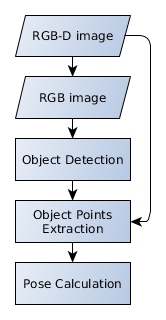
\includegraphics[width=\textwidth]{grasp_plan_pose_estimation}
        \caption{Pose estimation}
        \label{fig:grasp_plan_pose_estimation}
    \end{subfigure}
    \hfill  % add desired spacing between images, e. g. ~, \quad, \qquad, \hfill etc. 
            % (or a blank line to force the subfigure onto a new line)
    \begin{subfigure}[b]{0.55\textwidth}
        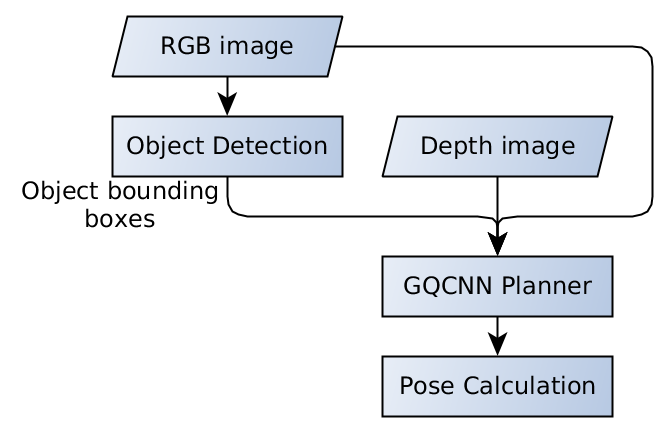
\includegraphics[width=\textwidth]{grasp_plan_gqcnn}
        \caption{GQCNN \cite{mahler2017}}
        \label{fig:grasp_plan_gqcnn}
    \end{subfigure}
    \caption{Pipelines of the two integrated approaches for planning grasps.}\label{fig:grasp_planners}
\end{figure}

For the baseline method, the grasp approach vector is assumed to align with the $ x $-axis of the robot base coordinate
frame, as illustrate in figure \ref{fig:base_link_frame}. This assumption reduces the 6-DOF grasp pose finding problem
to finding the 3D coordinates of the object.

\subsubsection*{Grasp detection with GQCNN}

\subsection{Grasp execution}

\pagebreak
\section{Experiment}

\picHereWidth{base_link_frame}{\texttt{base\_link} coordinate frame.}{fig:base_link_frame}{0.8\textwidth}

\picHereWidth{experimental_setup}
             {Experiment setup: the robot has the same starting pose facing the table before each grasp.}
             {fig:experiment_setup}{\textwidth}

\begin{figure}[htb]
    \centering
    \small
    \begin{subfigure}[b]{0.45\textwidth}
        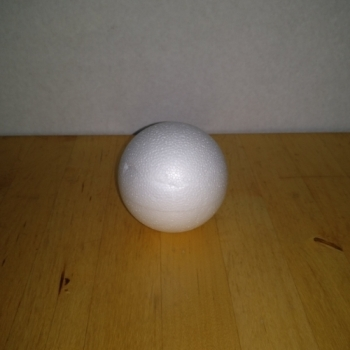
\includegraphics[width=\textwidth]{object_ball}
        \caption{A white styrofoam ball}
        \label{fig:object_ball}
    \end{subfigure}
    \hfill
    \begin{subfigure}[b]{0.45\textwidth}
        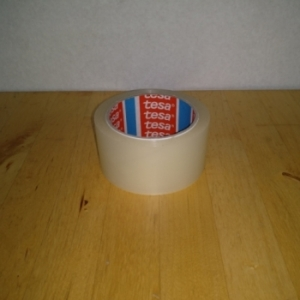
\includegraphics[width=\textwidth]{object_duct_tape}
        \caption{A roll of duct tape}
        \label{fig:object_duct_tape}
    \end{subfigure}

    \begin{subfigure}[b]{0.45\textwidth}
        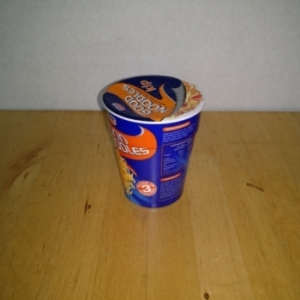
\includegraphics[width=\textwidth]{object_noodle_box}
        \caption{A cup noodles box}
        \label{fig:object_noodle_box}
    \end{subfigure}
    \hfill
    \begin{subfigure}[b]{0.45\textwidth}
    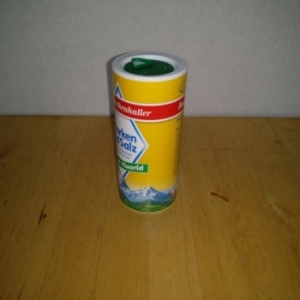
\includegraphics[width=\textwidth]{object_salt}
    \caption{A salt container}
    \label{fig:object_salt}
    \end{subfigure}
    \caption{Objects selected for the experiments.}\label{fig:objects}
\end{figure}

\subsection{Experiment setup}


\section{Results}

